\section{Experiments}
\label{sec:exp}
In this section, we first describe the dataset used in our paper. We then introduce all baselines and the evaluation metric. Finally, we present our research questions and results.

\subsection{Dataset}
\label{sec:dataset}
We used two well-known software projects (i.e., QT and OPENSTACK) to evaluate the performance of \emph{Just-In-Time} (JIT) models. QT~\footnote{\url{https://www.qt.io/}}, developed by the Qt Company, is a cross-platform application framework and allows contributions from individual developers and organizations. On the other hand, OPENSTACK~\footnote{\url{https://www.openstack.org/}} is an open-source software platform for cloud computing and is deployed as an infrastructure-as-a-service which allows customers to access its resources. 

\begin{table}[ht!]
  \centering
  \caption{Summary of the dataset used in this work}
    \begin{tabular}{|c|c|c|c|c|}
    \hline
    \multirow{2}[4]{*}{\textbf{Dataset}} & \multicolumn{2}{c|}{\textbf{Timespan}} & \multicolumn{2}{c|}{\textbf{Commits}} \\
\cline{2-5}          & \textbf{Start} & \textbf{End} & \textbf{Total} & \textbf{Defective} \\
    \hline
    \hline
    QT    & 06/2011 &  03/2014 & 25,150 & 2,002 (8\%) \\
    \hline
    OPENSTACK & 11/2011 &  02/2014 & 12,374 & 1,616 (13\%) \\
    \hline
    \end{tabular}%
  \label{tab:data}%
\end{table}%

Table~\ref{tab:data} briefly summarizes the dataset used in our paper. This dataset was originally collected and cleaned by McIntosh and Kamei~\cite{mcintosh2018fix}. After their cleaning process, the QT dataset contains 25,150 commits, while the OPENSTACK dataset contains 12,374 commits. McIntosh and Kamei stratified the dataset into six months periods for time-sensitive training-and-testing settings.

\subsection{Baselines}
\label{sec:baseline}

\begin{table*}[ht!]
	\centering
	\caption{A summary of McIntosh and Kamei's code features~\cite{mcintosh2018fix}.}
	\label{tab:metrics}
	\resizebox{\textwidth}{!}{
		\begin{tabular}{|c|p{2cm}|p{5.7cm}|p{8.4cm}|}
			\hline
			& {\bf Property} & {\bf Description} & {\bf Rationale} \\
			\hline
			\hline
			\multirow{2}{*}{\rotatebox{90}{Size}}
			& Lines deleted  & The number of deleted lines. &  The more deleted or added code, the more likely that defects \\
			\cline{2-3}
			& Lines added & The number of added lines. & may appear~\cite{nagappan2006icse}.\\
			\hline
			\multirow{4}{*}{\rotatebox{90}{Diffusion}}
			& Subsystems & The number of modified subsystems. & Scattered changes may have more defects compared to focused one~\cite{Ambros2010, HassanICSE09}.\\
			\cline{2-3}
			& Directories & The number of modified directories. & \\
			\cline{2-3}
			& Files & The number of modified files. &  \\
			\cline{2-3}
			& Entropy & The spread of modified lines across file. &  \\
			\hline
			\multirow{6}{*}{\rotatebox{90}{History}}
			& Unique changes & The number of prior changes to the modified files. & More changes may lead to have defects since developers need to track many previous changes~\cite{Kamei:2013:LES}.\\
			\cline{2-4}
			& Developers & The number of developers who have changed the modified files in the past. & Files touched by many developers may include defects~\cite{matsumoto2010promise}. \\
			\cline{2-4}
			& Age & The time interval between the last and current changes. & More recently changed code likely contains defects compared to older code~\cite{Graves2000}. \\
			\hline
			\multirow{11}{*}{\rotatebox{90}{Author/Rev. Experience}}
			& Prior changes & The number of prior changes that an actor has participated in. & Changes produced by novices are likely to be more defective than changes produced by experienced developers~\cite{Mockus2000}. \\
			\cline{2-3}
			& Recent changes & The number of prior changes that an actor has participated in weighted by the age of the changes (older changes are given less weight than recent ones). & \\
			\cline{2-3}
			& Subsystem changes & The number of prior changes to the modified subsystem(s) that an actor has participated in. & \\
			\cline{2-4}
			& Awareness & The proportion of the prior changes to the modified subsystem(s) that an actor has participated in. & Changes made by developers who are aware of the prior changes in the impacted subsystems are likely to be less risky. \\
			\hline
			\multirow{12}{*}{\rotatebox{90}{Review}}
			& Iterations & Number of times that a change was revised prior to integration. & The quality of a change likely improves with each iteration. Hence, changes that undergo iterations prior to integration may be less risky~\cite{porter1998tosem, thongtanunam2015msr}.\\
			\cline{2-4}
			& Reviewers & Number of reviewers who have voted on whether a change should be integrated or abandoned. & Changes observed by many reviewers are likely to be less risky~\cite{Raymond2001}. \\
			\cline{2-4}
			& Comments & The number of non-automated, non-owner comments posted during the review of a change. & Changes with short discussions may be more risky~\cite{mcintosh2014impact, mcintosh2016empirical}.\\
			\cline{2-4}
			& Review window & The length of time between the creation of a review request and its final approval for integration. & Changes with shorter review windows may be more risky~\cite{porter1998tosem, thongtanunam2015msr}.\\
			\hline
		\end{tabular}
	}
\end{table*}

We compared DeepJIT with two state-of-the-art baselines for \emph{Just-In-Time} (JIT) defect prediction:
\begin{itemize}
\item JIT: This method for identifying buggy code changes was proposed by McIntosh and Kamei~\cite{mcintosh2018fix}. The method used a nonlinear variant of multiple regression modeling~\cite{fox1997applied} to build a classification model for automatically identifying defects in commits. McIntosh and Kamei manually designed a set of code features, using six families of code change properties, which were primarily derived from prior studies~\cite{Kamei:2013:LES, Kim:2008:CSC, Kononenko:2015, Mockus2000}. These properties were: the magnitude of changes, the dispersion of the changes, the defect proneness of prior changes, the experience of the author, the code reviewers, and the degree of participation in the code review. Table~\ref{tab:metrics} briefly summarizes the code features extracted from code change properties.

\item DBNJIT: This approach adopted Deep Belief Network (DBN)~\cite{hinton2006reducing} to generate a more expressive set of features from an initial feature set~\cite{Yang:2015:DLJ}. The generated feature set, which is a nonlinear combination of the initial features, was put into a machine learning classifier~\cite{nasrabadi2007pattern} to predict buggy commits. For a fair comparison, we used McIntosh and Kamei~\cite{mcintosh2018fix}'s features as the initial feature set for DBNJIT. 
\end{itemize}

For all the above-mentioned techniques, we employ the same parameters and settings as described in the respective papers. 

\subsection{Evaluation Metric}
\label{sec:metric}
To evaluate the accuracy of \emph{Just-In-Time} (JIT) models, we calculate  threshold-independent measures of model performance. Since our dataset is imbalanced, we avoid using threshold-dependent measures (i.e., precision, recall, or F1) since these measures strongly depend on arbitraily thresholds~\cite{nguyen2009learning, gu2008data}. Following the previous work by McIntosh and Kamei~\cite{mcintosh2018fix}, we use the Area Under the receiver operator characteristics
Curve (AUC) to measure the discriminatory power of DeepJIT, i.e., their ability to differentiate between defective or clean commits. AUC computes the area under the curve plotting the true positive rate against the false positive rate, while applying multiple thresholds to determine if a commit is buggy or not. The values of AUC range between 0 (worst discrimination) and 1 (perfect discrimination).

\subsection{Training and hyperparameters}
\label{sec:training_parameters}
\begin{figure}[t!]
    \center
    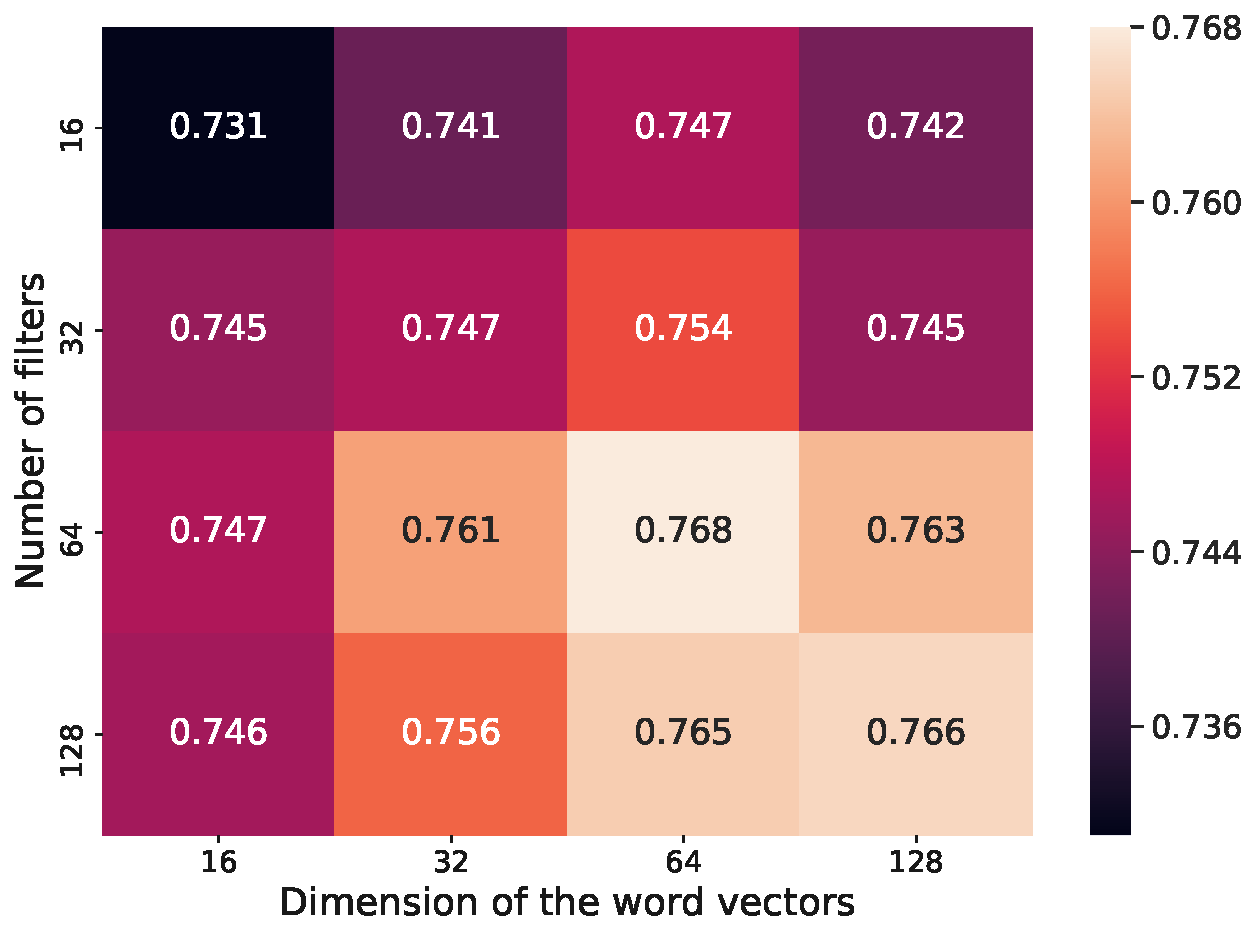
\includegraphics[width=\linewidth]{figs/QT.pdf}
    \caption{The AUC results of DeepJIT across two different hyperparameters in QT project.}
    \label{fig:qt}
\end{figure}
\begin{figure}[t!]
    \center
    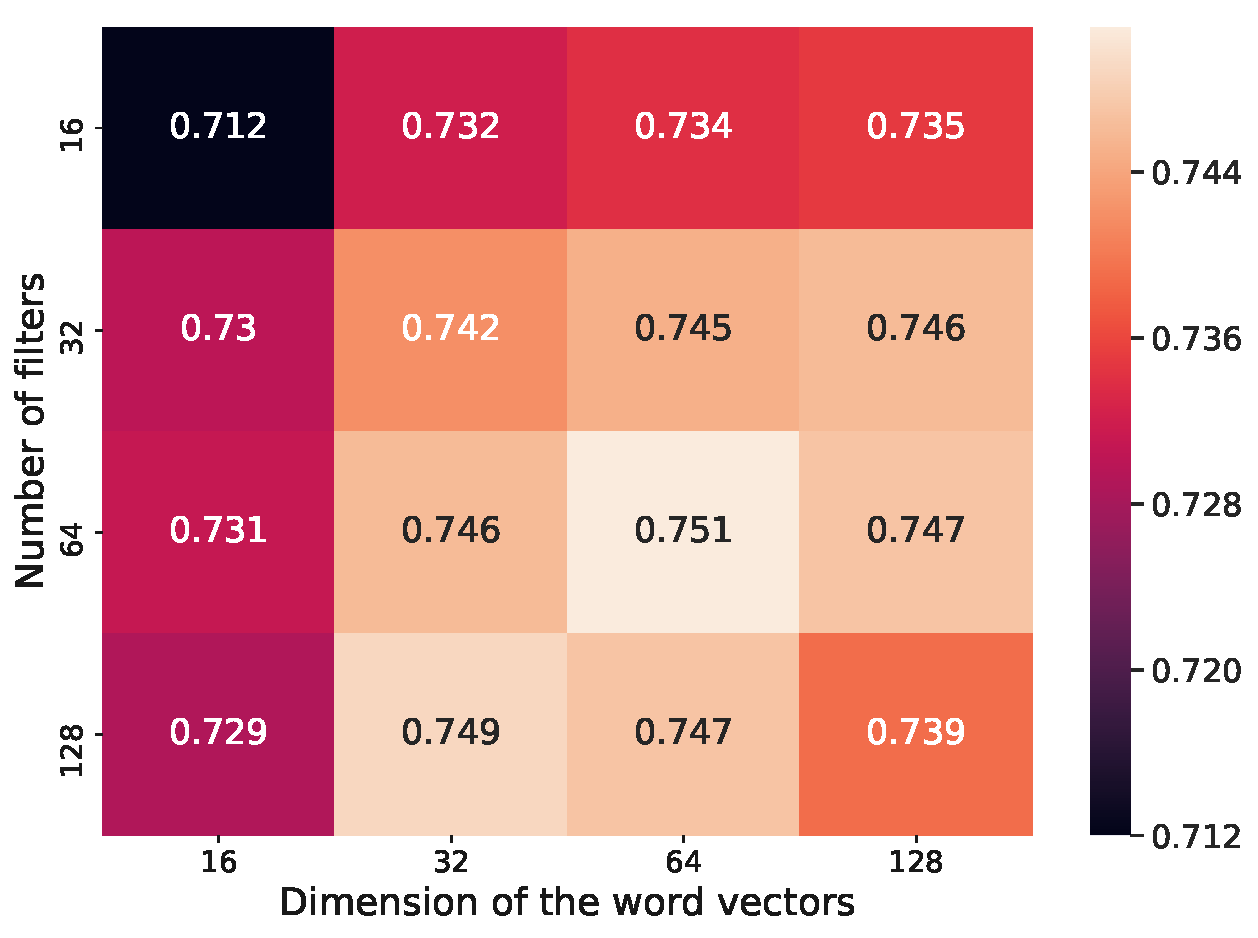
\includegraphics[width=\linewidth]{figs/OPENSTACK.pdf}
    \caption{The AUC results of DeepJIT across two different hyperparameters in OPENSTACK project.}
    \label{fig:openstack}
\end{figure}

One of the key challenges in training DeepJIT is how to select the dimension of the word vectors for the commit message ($d_m$) and code changes ($d_c$), and the size of the convolution layers (i.e., see Section~\ref{sec:cnn_msg} and Section~\ref{sec:cnn_code}). We evaluated the performance of DeepJIT, using \textit{5}-fold cross validation, across different word dimensions and number of filters. Figure~\ref{fig:qt} and Figure~\ref{fig:openstack} present the AUC results of DeepJIT for these hyperparameters. The figures show that DeepJIT achieves the best AUC results when the dimension of word vectors and the number of filters are set to 64. We set the other hyperparameters as follows: The batch size was set to 32. The size of DeepJIT's fully-connected layer described in Section~\ref{sec:ftr_combine} was set to 512. These hyperparameter settings are commonly used in prior deep learning work~\cite{severyn2015learning, huo2016learning, huo2017enhancing, hinton2012improving}.

We trained DeepJIT using Adam method~\cite{kingma2014adam} with shuffled mini-batches. We also trained DeepJIT for 100 epochs. We applied an early stopping strategy~\cite{prechelt1998automatic, caruana2001overfitting} to avoid overfitting problem during the training process. We stopped the training if the value of the objective function (see Equation~\ref{eq:cost}) has not been updated in the last 5 epochs. 

% For the size of the convolutional filters, we choose 64. The size of DeepJIT's fully-connected layer described in Section~\ref{sec:ftr_combine} is set to 512. The word vectors dimension of the commit message ($d_m$) and code changes ($d_c$) are set to 64. We train DeepJIT using Adam~\cite{kingma2014adam} with shuffled mini-batches.  The batch size is set to 32. We train DeepJIT for 100 epochs. We also apply the early stopping strategy~\cite{prechelt1998automatic, caruana2001overfitting} to avoid overfitting problem during the training process. Typically, we stop the training if the value of the objective function (see Equation~\ref{eq:cost}) has not been update in the last 5 epochs. All these hyperparameters in our paper are widely used in the deep learning community~\cite{severyn2015learning, huo2016learning, huo2017enhancing, hinton2012improving}. 
 
 

\subsection{Research Questions and Results}
\label{sec:rq_results}

\noindent \textbf{RQ1: How effective is DeepJIT compared to the state-of-the-art baseline?}

\begin{figure}
	\center
	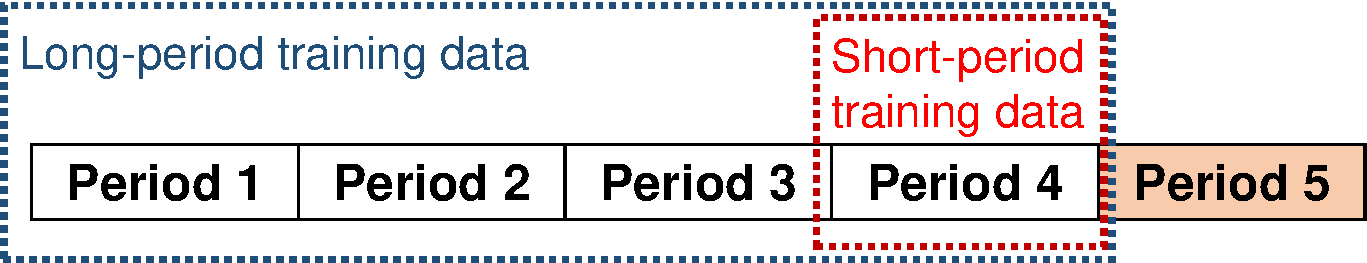
\includegraphics[scale=0.4]{figs/split.pdf}
	\caption{An example of choosing the training data for short-period and long-period models. The last period is used as testing data.}
	\label{fig:splitting}
\end{figure}

\begin{table}[ht]
  \centering
  \caption{The AUC results of DeepJIT vs. with other baselines in three types of JIT models: cross-validation, short-period, and long-period.}
    \begin{tabular}{|c|l|c|c|}
    \hline
    \textbf{Settings} & \multicolumn{1}{c|}{\textbf{Models}} & QT & OPENSTACK \\
    \hline
    \hline
    \multirow{3}[6]{*}{Cross-validation} & JIT   & 0.701 & 0.691 \\
\cline{2-4}          & DBNJIT & 0.705 & 0.694 \\
\cline{2-4}          & DeepJIT & \textbf{0.768} & \textbf{0.751} \\
    \hline
    \multirow{3}[6]{*}{Short-Period} & JIT   & 0.703 & 0.711 \\
\cline{2-4}          & DBNJIT & 0.714 & 0.716 \\
\cline{2-4}          & DeepJIT & \textbf{0.764} & \textbf{0.781} \\
    \hline
    \multirow{3}[6]{*}{Long-period} & JIT   & 0.702 & 0.706 \\
\cline{2-4}          & DBNJIT & 0.708 & 0.712 \\
\cline{2-4}          & DeepJIT & \textbf{0.765} & \textbf{0.771} \\
    \hline
    \end{tabular}%
  \label{tab:results}%
\end{table}%

To address RQ1, we evaluated the accuracy of a trained JIT model in predicting buggy changes using test data. In particular, we considered three evaluation settings: 
\begin{itemize}
\item \textbf{Cross-validation:} To evaluate machine learning algorithm, most people use $k$-fold cross-validation~\cite{kohavi1995study} in which a dataset is randomly divided to $k$ folds, each fold is considered as testing data for evaluating JIT model while $k - 1$ folds are considered as training data. In this case, the JIT model is trained on a mixture of past and future data. In our paper, we set $k = 5$.
\item \textbf{Short-period:} The JIT model is trained using commits that occurred at one time period. We assume that older commits changes may have characteristics that no longer effects to the latest commits. 
\item \textbf{Long-period:} Inspired by the work~\cite{rahman2013sample}, suggesting that larger amounts of training data tend to achieve a better performance in defect prediction problem, we train the JIT model using all commits that occurred before a particular period. We discover whether additional data may improve the performance of the JIT model. 
\end{itemize} 

Figure~\ref{fig:splitting} describes how the training data is selected to train models  following the short-period and long-period settings. We used the last period (i.e., period 5) as a testing data. While the short-period model was trained using the commits that occurred during period 4, the long-period model was trained using the commits that occurred from period 1 to 4. After training short-period and long-period models, we measured their performance using AUC evaluation metric described in Section~\ref{sec:metric}.

Table~\ref{tab:results} shows the AUC results of DeepJIT as well as other baselines considering the three evaluation settings: cross-validation, short-period, and long-period. The difference between results obtained using cross-validation, short-period, and long-period settings is relatively small (i.e., below 2.2\%) which suggests that there is no difference between training on past or future data. 
% \cmt{TODO: Prof. Hoa, do you have any explaination about it?} 
In the QT project, DeepJIT achieved AUC scores of 0.768, 0.764, and 0.765 in three different evaluation settings: cross-validation, short-period, and long-period, respectively. Comparing them to the best performing baseline (i.e., DBNJIT), DeepJIT achieved improvements of 8.96\%, 7.00\%, and 8.05\% in terms of AUC. In the OPENSTACK project, DeepJIT also constituted improvements of 8.21\%, 9.08\%, and 8.29\% in terms of AUC compared to DBNJIT (the best performing baseline). We also employed the Scott-Knott test~\cite{ghotra2015revisiting} on the cross-validation evaluation setting to statistically compare the differences between the three considered JIT models. The results show that DeepJIT consistently appears in the top Scott-Knott ESD rank in terms of AUC (i.e, DeepJIT $>$ DBNJIT $>$ JIT).  


\noindent \textbf{RQ2: Does the proposed model benefit from both commit message and the code changes?}

\begin{table}[ht!]
  \centering
  \caption{Contribution of feature components in DeepJIT.}
    \begin{tabular}{|c|l|c|c|}
    \hline
    \textbf{Settings} & \multicolumn{1}{c|}{\textbf{Models}} & QT & OPENSTACK \\
    \hline
    \hline
    \multirow{3}[6]{*}{Cross-validation} & DeepJIT-Msg & 0.641 & 0.689 \\
\cline{2-4}          & DeepJIT-Code & 0.738 & 0.729 \\
\cline{2-4}          & DeepJIT & \textbf{0.768} & \textbf{0.751} \\
    \hline
    \multirow{3}[6]{*}{Short-Period} & DeepJIT-Msg & 0.609 & 0.583 \\
\cline{2-4}          & DeepJIT-Code & 0.734 & 0.769 \\
\cline{2-4}          & DeepJIT & \textbf{0.764} & \textbf{0.781} \\
    \hline
    \multirow{3}[6]{*}{Long-period} & DeepJIT-Msg & 0.638 & 0.659 \\
\cline{2-4}          & DeepJIT-Code & 0.727 & 0.738 \\
\cline{2-4}          & DeepJIT & \textbf{0.765} & \textbf{0.771} \\
    \hline
    \end{tabular}%
  \label{tab:variants}%
\end{table}%

% \begin{table*}[t!]
%   \centering
%   \caption{Contribution of feature components in DeepJIT.}
%     \begin{tabular}{|l|c|c|c|c|c|c|}
%     \hline
%     \multirow{2}[4]{*}{} & \multicolumn{3}{c|}{QT} & \multicolumn{3}{c|}{OPENSTACK} \\
% \cline{2-7}          & \multicolumn{1}{l|}{\textbf{Cross-validation}} & \multicolumn{1}{l|}{\textbf{Short-period}} & \multicolumn{1}{l|}{\textbf{Long-period}} & \multicolumn{1}{l|}{\textbf{Cross-validation}} & \multicolumn{1}{l|}{\textbf{Short-period}} & \multicolumn{1}{l|}{\textbf{Long-period}} \\
%     \hline
%     \hline
%     DeepJIT-Msg & 0.641 & 0.609 & 0.638 & 0.689 & 0.583 & 0.659 \\
%     \hline
%     DeepJIT-Code & 0.738 & 0.734 & 0.727 & 0.729 & 0.769 & 0.738 \\
%     \hline
%     DeepJIT & \textbf{0.768} & \textbf{0.764} & \textbf{0.765} & \textbf{0.751} & \textbf{0.781} & \textbf{0.771} \\
%     \hline
%     \end{tabular}%
%   \label{tab:variants}%

% \end{table*}%

To answer this question, we employed an ablation test~\cite{korbar2017deep, liu2017deep}, by ignoring the commit message and the code change in a commit and then evaluate the AUC performance. Specifically, we created two different variants of DeepJIT, namely DeepJIT-Msg and DeepJIT-Code. DeepJIT-Msg only considers commit message information while DeepJIT-Code only uses commit code information. We again used the three evaluation settings (i.e., cross-validation, short-period, and long-period) and the AUC scores to evaluate the performance of our models. Table~\ref{tab:variants} shows the performance of DeepJIT degrades if we ignore any one of the considered types of information (i.e. commit messages or code changes). The AUC scores dropped by 19.81\%, 28.45\%, and 19.01\% in the project QT and dropped by 9.00\%, 33.96\%, and 16.00\% in the project OPENSTACK for the three evaluation settings if we ignore commit messages. The AUC scores dropped by 4.07\%, 4.09\%, and 5.23\% in the project QT and dropped by 3.02\%, 1.56\%, and 4.47\% in the project OPENSTACK for the three evaluation settings if we ignore code changes information. It suggests that each information type contributes to DeepJIT's performance. Moreover, it also indicates that code changes are more important to detect buggy commits than commit messages. 

\noindent \textbf{RQ3: Does DeepJIT benefit from the manually extracted code changes features?}

\begin{table}[ht]
  \centering
  \caption{Combination of DeepJIT with the manually crafted code features from~\cite{mcintosh2018fix}.}
    \begin{tabular}{|c|l|c|c|}
    \hline
    \textbf{Settings} & \multicolumn{1}{c|}{\textbf{Models}} & QT & OPENSTACK \\
    \hline
    \hline
    \multirow{2}[4]{*}{Cross-validation} & DeepJIT & 0.768 & 0.751 \\
\cline{2-4}          & DeepJIT-Combined & \textbf{0.779} & \textbf{0.76} \\
    \hline
    \multirow{2}[4]{*}{Short-Period} & DeepJIT & 0.764 & 0.781 \\
\cline{2-4}          & DeepJIT-Combined & \textbf{0.788} & \textbf{0.814} \\
    \hline
    \multirow{2}[4]{*}{Long-period} & DeepJIT & 0.765 & 0.771 \\
\cline{2-4}          & DeepJIT-Combined & \textbf{0.786} & \textbf{0.799} \\
    \hline
    \end{tabular}%
  \label{tab:combined}%
\end{table}%

To address this question, we incorporated the code features, derived from~\cite{mcintosh2018fix}, into our proposed model. Specifically, the code features, namely $\textbf{z}_\textbf{r}$, are concatenated with the two embedding vectors  $\textbf{z}_\textbf{m}$ and $\textbf{z}_C$, representing the salient features of commit message and code change (see Section~\ref{sec:ftr_combine}), to build a new single vector $\textbf{z}$ as follows:
\begin{equation}
\label{eq:combined_ftr}
\textbf{z} = \textbf{z}_\textbf{m} \oplus \textbf{z}_C \oplus \textbf{z}_\textbf{r}
\end{equation}
where $\oplus$ is the concatenation operator. Table~\ref{tab:combined} shows the AUC results of a DeepJIT variant (referred to as DeepJIT-Combined) that also leverages McIntosh and Kamei~\cite{mcintosh2018fix}'s manually crafted features. We find that the AUC scores increased by 1.43\%, 3.14\%, and 2.75\% in the project QT and they increased by 1.20\%, 4.23\%, and 3.63\% in the project OPENSTACK for the three evaluation settings (i.e. cross-validation, short-period, long-period). DeepJIT-Combined improved the best baseline model (i.e. DBNJIT) by 10.50\%, 10.36\%, and 11.02\% in the project QT and 9.51\%, 13.69\%, 12.22\% in the project OPENSTACK for the there evaluation settings. This suggests that the manually extracted code features are complementary and can be used to improve the performance of our proposed approach.

\noindent \textbf{RQ4: What are the time costs of DeepJIT?}
% \begin{table*}[t!]
%   \centering
%   \caption{Time costs of DeepJIT.}
%     \begin{tabular}{|c|c|c|c|c|c|c|}
%     \hline
%     \multicolumn{1}{|c|}{\multirow{2}[4]{*}{Dataset}} & \multicolumn{2}{c|}{\textbf{Cross-validation}} & \multicolumn{2}{c|}{\textbf{Short-period}} & \multicolumn{2}{c|}{\textbf{Long-period}} \\
% \cline{2-7}          & Training time & Testing time & Training time & Testing time & Training time & Testing time \\
%     \hline
%     \hline
%     QT    & 5 hours 43 mins & 36.2 mins & 17.2 mins & 3.2 mins & 1 hours 18 mins & 8.1 mins \\
%     \hline
%     OPENSTACK & 12 hours 15 mins & 1 hours 6 mins & 10.1 mins & 2.3 mins & 2 hours 37 mins & 12.4 mins \\
%     \hline
%     \end{tabular}%
%   \label{tab:cost}%
% \end{table*}%

\begin{table}[t!]
  \centering
  \caption{Training time of DeepJIT}
    \begin{tabular}{|l|c|c|c|}
    \hline
    \multicolumn{1}{|c|}{Dataset} & Cross-validation & Short-period & Long-period \\
    \hline
    \hline
    QT    & 5 hours 43 mins & 17.2 mins & 1 hours 18 mins \\
    \hline
    OPENSTACK & 12 hours 15 mins & 10.1 mins & 2 hours 37 mins \\
    \hline
    \end{tabular}%
  \label{tab:cost}%
\end{table}%

We trained and tested DeepJIT on a NVIDIA DGX1 server with Tesla P100~\cite{gawande2018scaling}. Table~\ref{tab:cost} shows the time costs of training DeepJIT for the three evaluation settings (i.e., cross-validation, short-period, and long-period) on QT and OPENSTACK. Cross-validation setting requires longest training time since we performed $5$-fold cross-validation to evaluate the performance of DeepJIT. Long-period setting requires more training time than short-period setting since it considers all commits occurring before a particular period. Once DeepJIT has been trained, it only takes a few milliseconds to generate the prediction score for a given commit.
% \cmt{Prof. Hoa: do you have any idea how to describe the time cost?}

